Feature selection was performed in the exact same way as in case of noise-free images, meaning by a a stepwise regression algorithm with five steps forward and three steps backward. As a result of this process from a set of 196 available features, 10 features were used. Figures \ref{fig:nonlinear_noised_features_colour} and \ref{fig:nonlinear_noised_features_percentage} depicts which features were chosen for this experiment in the same way as in case of the previous experiment. When it comes to grid colour features only two were chosen, which is four less than in case of the optimal feature set for segmentation of noise-free images. However, the chosen two features, which are are the colour of the superpixel under consideration, and the colour of a middle superpixel in the bottom row of the grid were also a part of a feature set used in the previous experiment. When it comes to features of neighbour colour percentages, two less features were chosen comparing to a noise-free case. Once again, a percentage of green neighbours of the superpixel under consideration is taken into account. There are also two other features of green neighbours percentage that were chosen for both, noise-free and noised data. 
\begin{figure}
    \centering
    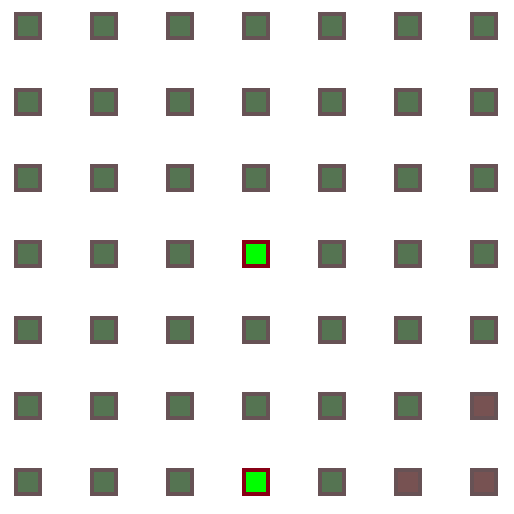
\includegraphics[width=0.5\textwidth]{nonlinear_noised/features/grid_colour_chosen_noised.png}
    \caption{Chosen grid colour features for experiments on noised data}
    \label{fig:nonlinear_noised_features_colour}
\end{figure}
\begin{figure}
    \centering
    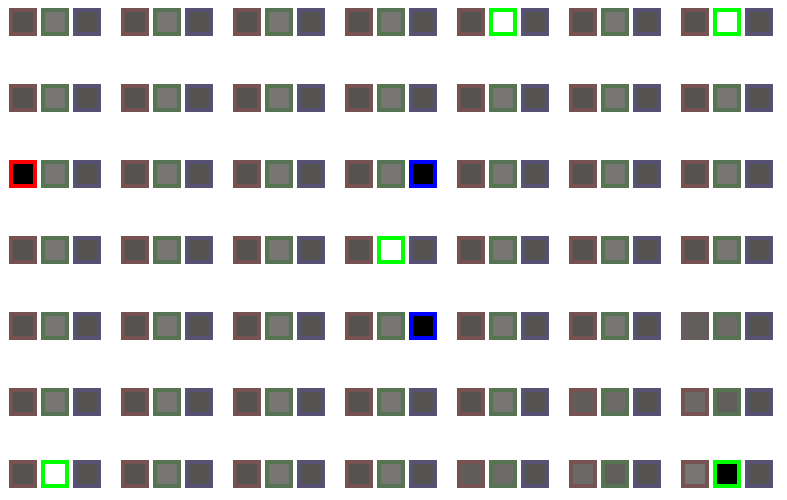
\includegraphics[width=\textwidth]{nonlinear_noised/features/grid_colour_percentage_chosen_noised.png}
    \caption{Chosen grid neighbour colour percentage features for experiments on noised data.}
    \label{fig:nonlinear_noised_features_percentage}
\end{figure}




In order to proof the importance of proper feature selection figures \ref{fig:noised_fi1_all_features} and \ref{fig:noised_fi1_selected_features} were prepared. Both figures show probabilities $p(y|x)$ of each label for 3 test samples, however, the first one presents the results if all 196 features were used, and the second one if a a set of 10 selected features only. As visible, for a set of all 

\begin{figure}
    \renewcommand{\arraystretch}{4}
    \begin{tabular}{cccc}
        \textit{test image} &
        \fcolorbox{black}{white}{\includegraphics[align=c,width= 0.22\textwidth]{nonlinear_noised/fi1_all_features/1/image.png}} &
        \fcolorbox{black}{white}{\includegraphics[align=c,width= 0.22\textwidth]{nonlinear_noised/fi1_all_features/2/image.png}} &
        \fcolorbox{black}{white}{\includegraphics[align=c,width= 0.22\textwidth]{nonlinear_noised/fi1_all_features/3/image.png}}  \\
        \textit{label 0} &
        \fcolorbox{black}{white}{\includegraphics[align=c,width= 0.22\textwidth]{nonlinear_noised/fi1_all_features/1/label_0.png}} &
        \fcolorbox{black}{white}{\includegraphics[align=c,width= 0.22\textwidth]{nonlinear_noised/fi1_all_features/2/label_0.png}} &
        \fcolorbox{black}{white}{\includegraphics[align=c,width= 0.22\textwidth]{nonlinear_noised/fi1_all_features/3/label_0.png}} \\
        \textit{label 1} &
        \fcolorbox{black}{white}{\includegraphics[align=c,width= 0.22\textwidth]{nonlinear_noised/fi1_all_features/1/label_1.png}} &
        \fcolorbox{black}{white}{\includegraphics[align=c,width= 0.22\textwidth]{nonlinear_noised/fi1_all_features/2/label_1.png}} &
        \fcolorbox{black}{white}{\includegraphics[align=c,width= 0.22\textwidth]{nonlinear_noised/fi1_all_features/3/label_1.png}} \\
        \textit{label 2} &
        \fcolorbox{black}{white}{\includegraphics[align=c,width= 0.22\textwidth]{nonlinear_noised/fi1_all_features/1/label_2.png}} &
        \fcolorbox{black}{white}{\includegraphics[align=c,width= 0.22\textwidth]{nonlinear_noised/fi1_all_features/2/label_2.png}} &
        \fcolorbox{black}{white}{\includegraphics[align=c,width= 0.22\textwidth]{nonlinear_noised/fi1_all_features/3/label_2.png}} \\
        \textit{label 3} &
        \fcolorbox{black}{white}{\includegraphics[align=c,width= 0.22\textwidth]{nonlinear_noised/fi1_all_features/1/label_3.png}} &
        \fcolorbox{black}{white}{\includegraphics[align=c,width= 0.22\textwidth]{nonlinear_noised/fi1_all_features/2/label_3.png}} &
        \fcolorbox{black}{white}{\includegraphics[align=c,width= 0.22\textwidth]{nonlinear_noised/fi1_all_features/3/label_3.png}}
    \end{tabular}
    \caption{Visual representation of conditional probabilities $p(y|x)$ for noised images without feature selection.}
    \label{fig:noised_fi1_all_features}
\end{figure}


\begin{figure}
 \renewcommand{\arraystretch}{4}
    \begin{tabular}{cccc}
        \textit{test image} &
        \fcolorbox{black}{white}{\includegraphics[align=c,width= 0.22\textwidth]{nonlinear_noised/fi1_selected_features/1/image.png}} &
        \fcolorbox{black}{white}{\includegraphics[align=c,width= 0.22\textwidth]{nonlinear_noised/fi1_selected_features/2/image.png}} &
        \fcolorbox{black}{white}{\includegraphics[align=c,width= 0.22\textwidth]{nonlinear_noised/fi1_selected_features/3/image.png}}  \\
        \textit{label 0} &
        \fcolorbox{black}{white}{\includegraphics[align=c,width= 0.22\textwidth]{nonlinear_noised/fi1_selected_features/1/label_0.png}} &
        \fcolorbox{black}{white}{\includegraphics[align=c,width= 0.22\textwidth]{nonlinear_noised/fi1_selected_features/2/label_0.png}} &
        \fcolorbox{black}{white}{\includegraphics[align=c,width= 0.22\textwidth]{nonlinear_noised/fi1_selected_features/3/label_0.png}} \\
        \textit{label 1} &
        \fcolorbox{black}{white}{\includegraphics[align=c,width= 0.22\textwidth]{nonlinear_noised/fi1_selected_features/1/label_1.png}} &
        \fcolorbox{black}{white}{\includegraphics[align=c,width= 0.22\textwidth]{nonlinear_noised/fi1_selected_features/2/label_1.png}} &
        \fcolorbox{black}{white}{\includegraphics[align=c,width= 0.22\textwidth]{nonlinear_noised/fi1_selected_features/3/label_1.png}} \\
        \textit{label 2} &
        \fcolorbox{black}{white}{\includegraphics[align=c,width= 0.22\textwidth]{nonlinear_noised/fi1_selected_features/1/label_2.png}} &
        \fcolorbox{black}{white}{\includegraphics[align=c,width= 0.22\textwidth]{nonlinear_noised/fi1_selected_features/2/label_2.png}} &
        \fcolorbox{black}{white}{\includegraphics[align=c,width= 0.22\textwidth]{nonlinear_noised/fi1_selected_features/3/label_2.png}} \\
        \textit{label 3} &
        \fcolorbox{black}{white}{\includegraphics[align=c,width= 0.22\textwidth]{nonlinear_noised/fi1_selected_features/1/label_3.png}} &
        \fcolorbox{black}{white}{\includegraphics[align=c,width= 0.22\textwidth]{nonlinear_noised/fi1_selected_features/2/label_3.png}} &
        \fcolorbox{black}{white}{\includegraphics[align=c,width= 0.22\textwidth]{nonlinear_noised/fi1_selected_features/3/label_3.png}}
    \end{tabular}
    \caption{Visual representation of conditional probabilities $p(y|x)$ for noised images after feature selection.}
    \label{fig:noised_fi1_selected_features}
\end{figure}